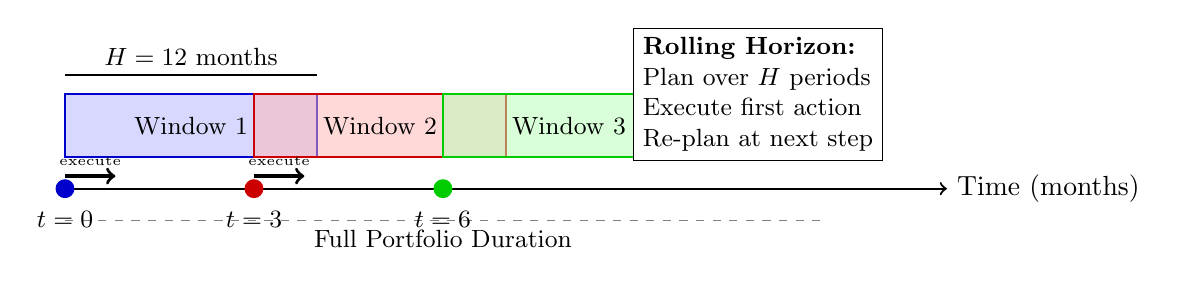
\begin{tikzpicture}[scale=0.8]
    % Timeline
    \draw[thick, ->] (0,0) -- (14,0) node[right] {Time (months)};
    
    % Full horizon indicator
    \draw[dashed, gray] (0,-0.5) -- (12,-0.5);
    \node[below] at (6,-0.5) {\small Full Portfolio Duration};
    
    % Rolling windows
    % Window 1
    \fill[blue!30, opacity=0.5] (0,0.5) rectangle (4,1.5);
    \draw[thick, blue!80!black] (0,0.5) rectangle (4,1.5);
    \node at (2,1) {\small Window 1};
    \fill[blue!80!black] (0,0) circle (0.15);
    \node[below] at (0,-0.2) {\small $t=0$};
    
    % Window 2
    \fill[red!30, opacity=0.5] (3,0.5) rectangle (7,1.5);
    \draw[thick, red!80!black] (3,0.5) rectangle (7,1.5);
    \node at (5,1) {\small Window 2};
    \fill[red!80!black] (3,0) circle (0.15);
    \node[below] at (3,-0.2) {\small $t=3$};
    \draw[->, very thick] (0,0.2) -- (0.8,0.2) node[midway, above, font=\tiny] {execute};
    
    % Window 3
    \fill[green!30, opacity=0.5] (6,0.5) rectangle (10,1.5);
    \draw[thick, green!80!black] (6,0.5) rectangle (10,1.5);
    \node at (8,1) {\small Window 3};
    \fill[green!80!black] (6,0) circle (0.15);
    \node[below] at (6,-0.2) {\small $t=6$};
    \draw[->, very thick] (3,0.2) -- (3.8,0.2) node[midway, above, font=\tiny] {execute};
    
    % Planning horizon bracket
    \draw[thick] (0,1.8) -- (4,1.8);
    \node[above] at (2,1.8) {\small $H=12$ months};
    
    % Legend
    \node[draw, fill=white, align=left, font=\small] at (11,1.5) {
        \textbf{Rolling Horizon:}\\
        Plan over $H$ periods\\
        Execute first action\\
        Re-plan at next step
    };
\end{tikzpicture}
